\expandafter\let\csname ver@amssymb.sty\endcsname\empty
\documentclass[serif]{beamer}
\expandafter\let\csname ver@amssymb.sty\endcsname\relax
\usepackage{etex}
\usepackage[bitstream-charter]{mathdesign} % Use BT Charter font
\usepackage[T1]{fontenc}                   % Use T1 encoding instead of OT1
\usepackage[utf8]{inputenc}                % Use UTF8 input encoding
\usepackage{microtype}                     % Improve typography
\usepackage{booktabs}
\usepackage{cancel}
\usepackage{algorithm}
\usepackage{algorithmicx}
\usepackage{algpseudocode}
\usepackage{hyperref}
\hypersetup{pdfstartview=Fit}
\usepackage{tikz}
\usetikzlibrary{shapes,snakes,shadows,arrows,calc,decorations.markings}
\usepackage{multirow}
\usepackage{animate}
\usepackage{moresize}
\usepackage{colortbl}
\usepackage{xcolor}
\usepackage{amsmath}
\usepackage{etoolbox}
\usepackage{listings}
\usepackage{alltt}

\renewcommand\footnotemark{}

\lstset{
  columns=fullflexible,
  showspaces=false,
  showtabs=false,
  showstringspaces=false,
  commentstyle=\color{gray}\upshape,
}
\lstset{language=bash,frame=single,basicstyle=\ttfamily\footnotesize}
\lstdefinelanguage{XML}
{
  backgroundcolor=\color{gray!20},
  basicstyle=\ttfamily\ssmall,
  morestring=[b]",
  frame=single,
% morestring=[s]{>}{<},
  morecomment=[s]{<?}{?>},
  morecomment=[s]{<!--}{-->},
  stringstyle=\color{red},
  identifierstyle=\color{darkblue},
  keywordstyle=\color{cyan},
}

\definecolor{gray}{rgb}{0.4,0.4,0.4}
\definecolor{darkblue}{rgb}{0.0,0.0,0.6}
\definecolor{cyan}{rgb}{0.0,0.6,0.6}

\newcommand{\tikzmark}[1]{\tikz[overlay,remember picture] \node (#1) {};}
\newcommand*{\DrawArrow}[3][]{%
    % #1 = draw options
    % #2 = left point
    % #3 = right point
    \begin{tikzpicture}[overlay,remember picture]
        \draw [-latex, #1] ($(#2)+(0.3em,0.5ex)$) to ($(#3)+(0,0.5ex)$);
    \end{tikzpicture}%
}

\usetheme{Copenhagen}
\usecolortheme{beaver}

\title{OpenMC Module: Monte Carlo Theory}
\author{\emph{Computational Reactor Physics Group}}
\date{\normalsize Department of Nuclear Science and Engineering\\
                  Massachusetts Institute of Technology}
% Set Logo
\logo{
\includegraphics[scale=0.2]{../src/crpg.png}\hspace*{8cm}

\includegraphics[scale=0.2,trim=0cm 3.0cm 2.2cm 0cm, clip=true]{../src/mitlogo.pdf}}

\usenavigationsymbolstemplate{}

\newcommand{\proton}[1]{%
    \shade[ball color=red] (#1) circle (.25);\draw (#1) node{$+$};
}

%\neutron{xposition,yposition}
\newcommand{\neutron}[1]{%
    \shade[ball color=green] (#1) circle (.25);
}

\newcommand{\nucleus}{%
    \neutron{0.1,0.3}
    \proton{0,0}
    \neutron{0.3,0.2}
    \proton{-0.2,0.1}
    \neutron{-0.1,0.3}
    \proton{0.2,-0.15}
    \neutron{-0.05,-0.12}
    \proton{0.17,0.21}
}

% For Loop 
\newcommand{\forloop}[5][1]% 
{% 
\setcounter{#2}{#3}% 
\ifthenelse{#4}% 
  {% 
  #5% 
  \addtocounter{#2}{#1}% 
  \forloop[#1]{#2}{\value{#2}}{#4}{#5}%
  }% 
% Else 
  {% 
  }% 
}%


%-------------------------------------------------------------------------------
\begin{document}
%-------------------------------------------------------------------------------

\frame{\titlepage}\logo{} % remove logo after title page

%-------------------------------------------------------------------------------

\begin{frame}{Solving the Neutron Transport Equation}

  \begin{itemize}
    \item<1-> Assume $\partial\psi / \partial t = 0$ and scale fission term
      \begin{equation*}
        \begin{split}
          \hat{\Omega} \cdot \nabla \psi_k &+ \Sigma_t(\mathbf{r},E)
          \psi_k(\mathbf{r},\hat\Omega,E) = \\ &\iint dE' d\Omega'
          \Sigma_s(\mathbf{r},\hat\Omega\cdot\hat\Omega',E'\to
          E)\psi_k(\mathbf{r},\hat\Omega',E') \\ &+ \frac{1}{k} \frac{\chi(E)}{4\pi}
          \int dE' \nu \Sigma_f(\mathbf{r},E')\phi_k(\mathbf{r},E')
        \end{split}
      \end{equation*}\vfill
    \item<1-> Eigenvalue problem for $k$ and $\psi_k$\vfill
    \item<1-> Monte Carlo method invovles simulating individual neutrons\vfill
    \item<1-> Random numbers are sampled from probability distributions that
              represent physics 
  \end{itemize}

\end{frame}

%-------------------------------------------------------------------------------

\begin{frame}{Cross Section Data Needed}

  \begin{itemize}
    \item<1-> Microscopic cross sections and other physics laws are input into
              Monte Carlo codes\vfill
    \item<1-> Data contained in ACE-formatted files\vfill
    \item<1-> These files are commonly generated with NJOY proecessing code\vfill
    \item<1-> Currently can be obtained via MCNP/Serpent Software
    \vfill
    \begin{center}
      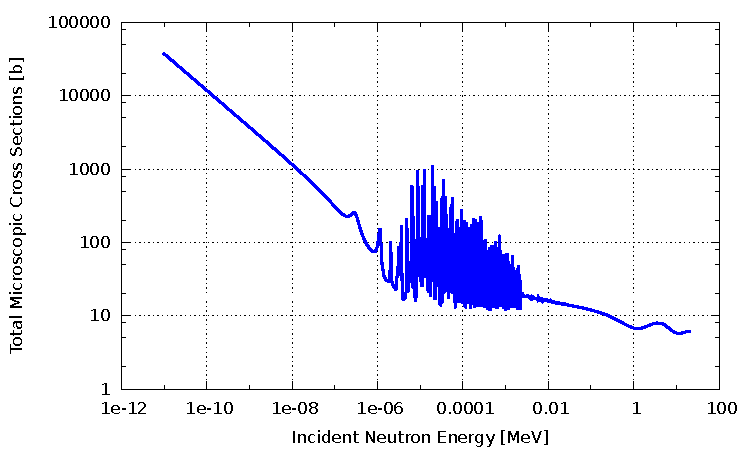
\includegraphics[scale=0.55]{../src/U235xs.pdf}
    \end{center}
  \end{itemize}

\end{frame}

%-------------------------------------------------------------------------------

\begin{frame}{Basic Monte Carlo Algorithm -- Eigenvalue}
    \begin{algorithmic}
      \State Guess initial source distribution and $k$
        \For {$i = 1 \to n_{batches}$}
          \For {$j =1 \to n_{particles}$}
            \State Sample neutron from source distribution
            \While {Neutron is alive}
              \State Sample distance to collision
              \State Determine isotope in collision
              \State Sample physics
              \State Bank fission sites
            \EndWhile
          \EndFor
          \State Sample neutrons from fission sites collected
          \State Calculate $k$
        \EndFor
    \end{algorithmic}
\end{frame}

%-------------------------------------------------------------------------------

\begin{frame}{Distance to Neutron Collision}

\begin{columns}
\begin{column}{0.5\linewidth}
\only<1,3->{
\begin{tikzpicture}
  \shade[shading=axis, bottom color=red, top color=white, shading angle=90] (-3.0cm,0.0cm) rectangle (0.0cm,4.0cm);
  \shade[shading=axis, bottom color=blue, top color=white, shading angle=-90] (0.0cm,0.0cm) rectangle (3.0cm,4.0cm);
  \node at (-1.5cm,3.75cm) {Region 1};
  \node at ( 1.5cm,3.75cm) {Region 2};
  \draw[<->,very thick] (-3.0cm,0.0cm) -- (3.0cm,0.0cm);
  \draw[very thick] (0.0cm,0.0cm) -- (0.0cm,4.0cm);
        \tikzstyle{nucleon}=[shape = circle, shading=ball,
                             minimum size=0.25cm, ball color=green];
        \tikzstyle{nucleonblack}=[draw=black, fill=black,shape = circle,
                             minimum size=0.25cm, color=black];

        \node[nucleon] at (-2.8cm,0.3cm) {};
  \only<3->{
        \node[nucleonblack] at (-2.8cm,0.3cm) {};
  }
  \only<3>{
        \draw[->,color=orange,very thick] (-2.6cm,0.35cm) -- (2.0cm,1.5cm);
        \node[nucleon] at (2.2cm,1.58cm) {};
  }
  \only<4->{
        \node[nucleonblack] at (2.2cm,1.58cm) {};
        \draw[dashed,color=gray,very thick] (-2.6cm,0.35cm) -- (0.0cm,1.0cm);
  }
  \only<4>{
        \draw[->,color=orange,very thick] (2.0cm,1.5cm) -- (0.2cm,1.05cm);
        \node[nucleon] at (0.0cm,1.0cm) {};
  }
  \only<5->{
        \draw[dashed,color=gray,very thick] (2.0cm,1.5cm) -- (0.2cm,1.05cm);
        \node[nucleonblack] at (0.0cm,1.0cm) {};
  }
  \only<5>{
        \draw[->,color=orange,very thick] (0.2cm,1.05cm) -- (1.15cm,1.3cm);
        \node[nucleon] at (1.3cm,1.33cm) {};
  }
\end{tikzpicture}
}
\only<2>{
\begin{tikzpicture}[domain=0:4]
    \draw[very thin,color=gray] (-0.1,-1.1) grid (3.9,3.9);
    \draw[->] (-0.2,0) -- (4.2,0) node[right] {$x$};
    \draw[->] (0,-1.2) -- (0,4.2) node[above] {$p(x)$};
    \fill[fill=yellow!20] plot[id=exp] function{3.0*exp(-x)} --
    (4,0) -- (0,0) -- cycle;
    \draw[color=red] plot[id=exp] function{3.0*exp(-x)};
\end{tikzpicture}}
\end{column}
\begin{column}{0.5\linewidth}

  \begin{itemize}
    \item {\only<1>{\color{red}}Neutron is born or exits collision}\vfill
    \item {\only<2>{\color{red}}Neutrons are sampled from:
    \[ p(x)dx = \Sigma_t e^{-\Sigma_t x}dx\]}
    \vfill
    \item {\only<3>{\color{red}}If a surface is crossed}, {\only<4>{\color{red}}neutron is resampled from this surface}\vfill
    \item {\only<5>{\color{red}}If a surface is not crossed, a neutron has collided}
  \end{itemize}

\end{column}
\end{columns}

\end{frame}

%-------------------------------------------------------------------------------

\begin{frame}{Choosing the isotope involved in collision}
\begin{center}
\scalebox{0.8}{
\begin{tikzpicture}

        \tikzstyle{nucleon}=[shape = circle, shading=ball, 
                             minimum size=0.25cm, ball color=green];
        \tikzstyle{isotope}=[shape = circle, shading=ball, 
                             minimum size=1.00cm, ball color=red];
        \coordinate (N1) at (-2.0cm,0.0cm);
        \coordinate (I1) at (2.0cm,2.0cm);
        \coordinate (I2) at (2.0cm,0.0cm);
        \coordinate (I3) at (2.0cm,-2.0cm);
    
        % Draw coils
        \draw[snake=coil,segment aspect=0,very thick,segment length=20pt,
              line before snake=1mm,line after snake=1mm,->,draw=black!50]
              (N1) -> (1.5cm,1.7cm) node [pos=0.5,yshift=0.1cm] {\color{orange}?};
        \draw[snake=coil,segment aspect=0,very thick,segment length=20pt,
              line before snake=1mm,line after snake=1mm,->,draw=black!50]
              (N1) -> (1.4cm,0.0cm) node [pos=0.5,yshift=0.1cm] {\color{orange}?};
        \draw[snake=coil,segment aspect=0,very thick,segment length=20pt,
              line before snake=1mm,line after snake=1mm,->,draw=black!50]
              (N1) -> (1.5cm,-1.8cm) node [pos=0.5,yshift=0.1cm] {\color{orange}?};

        % Draw incoming neutron
        \node[nucleon] at (N1) {n};
        \node[isotope] at (I1) {U235};
        \node[isotope] at (I2) {U238};
        \node[isotope] at (I3) {O16};

\end{tikzpicture}}
\vfill
\begin{itemize}
  \item Select random number (0,1), $\xi$ \tikzmark{start}
\end{itemize}
\vfill
\begin{tikzpicture}
  \shade[shading=axis, bottom color=blue, top color=white, shading angle=0] (-5.0cm,0.0cm) rectangle (-1.0cm,0.2cm);
  \shade[shading=axis, bottom color=red, top color=white, shading angle=0] (-1.0cm,0.0cm) rectangle (2.0cm,0.2cm);
  \shade[shading=axis, bottom color=green, top color=white, shading angle=0] (2.0cm,0.0cm) rectangle (5.0cm,0.2cm);
  \node at (-3.0cm,0.0cm) {\tikzmark{end}};
  \draw[color=black,very thick] (-5.0cm,0.0cm) -- (5.0cm,0.0cm);
  \draw[color=black,very thick] (-5.0cm,-0.1cm) -- (-5.0cm,0.1cm) node [yshift=-0.4cm] {0.0};
  \draw[color=black,very thick] (5.0cm,-0.1cm) -- (5.0cm,0.1cm) node [yshift=-0.4cm] {1.0};
  \draw[color=black,very thick] (-1.0cm,-0.1cm) -- (-1.0cm,0.1cm) node [yshift=-0.5cm] {$\frac{\Sigma_{U238}}{\sum_i\Sigma_i}$};
  \draw[color=black,very thick] (2.0cm,-0.1cm) -- (2.0cm,0.1cm) node [yshift=-0.5cm] {$\frac{\Sigma_{U238}+\Sigma_{U235}}{\sum_i\Sigma_i}$};
  \node at (-3.0cm,-0.4cm) {U-238};
  \node at (0.5cm,-0.4cm) {U-235};
  \node at (3.5cm,-0.4cm) {O-16};
\end{tikzpicture}
\DrawArrow[orange, thick, out=-30, in=30]{start}{end}
\end{center}
\end{frame}

%-------------------------------------------------------------------------------

\begin{frame}{Sampling the Interaction Physics}

\begin{center}
\scalebox{0.8}{
\begin{tikzpicture}

    
        % Draw coils
        \draw[snake=coil,segment aspect=0,very thick,segment length=20pt,
              line before snake=1mm,line after snake=1mm,->,draw=black!50]
              (-4.0,0.5) -> (-1.0,0.0);
        \draw[snake=coil,segment aspect=0,very thick,segment length=20pt,
              line before snake=1mm,line after snake=1mm,->,draw=black!50]
              (0.0,0.0) -> (2.0,-2.0);
        % Draw incoming neutron
        \nucleus
        \neutron{-4.0,0.5}
        \neutron{2.2,-2.2}

\end{tikzpicture}}
\vfill
\begin{itemize}
  \item Select random number (0,1), $\xi$ \tikzmark{start}
\end{itemize}
\vfill
\begin{tikzpicture}
  \shade[shading=axis, bottom color=blue, top color=white, shading angle=0] (-5.0cm,0.0cm) rectangle (-3.0cm,0.2cm) node at (-4.0cm,0.2cm) {elastic};
  \shade[shading=axis, bottom color=red, top color=white, shading angle=0] (-3.0cm,0.0cm) rectangle (0.0cm,0.2cm) node at (-1.5cm,0.2cm) {inelastic};
  \shade[shading=axis, bottom color=green, top color=white, shading angle=0] (0.0cm,0.0cm) rectangle (2.0cm,0.2cm) node at (1.0cm,0.13cm) {capture};
  \shade[shading=axis, bottom color=orange, top color=white, shading angle=0] (2.0cm,0.0cm) rectangle (5.0cm,0.2cm) node at (3.5cm,0.2cm) {other rxns};
  \node at (-0.2cm,0.0cm) {\tikzmark{end}};
  \draw[color=black,very thick] (-5.0cm,0.0cm) -- (5.0cm,0.0cm);
  \draw[color=black,very thick] (-5.0cm,-0.1cm) -- (-5.0cm,0.1cm) node [yshift=-0.4cm] {0.0};
  \draw[color=black,very thick] (5.0cm,-0.1cm) -- (5.0cm,0.1cm) node [yshift=-0.4cm] {1.0};
  \draw[color=black,very thick] (-3.0cm,-0.1cm) -- (-3.0cm,0.1cm) node [yshift=-0.5cm] {$\frac{\sigma_{el}}{\sigma_t}$};
  \draw[color=black,very thick] (0.0cm,-0.1cm) -- (0.0cm,0.1cm) node [yshift=-0.5cm] {$\frac{\sigma_{el}+\sigma_{in}}{\sigma_t}$};
  \draw[color=black,very thick] (0.0cm,-0.1cm) -- (0.0cm,0.1cm) node [yshift=-0.5cm] {$\frac{\sigma_{el}+\sigma_{in}}{\sigma_t}$};
  \draw[color=black,very thick] (2.0cm,-0.1cm) -- (2.0cm,0.1cm) node [yshift=-0.5cm] {$\frac{\sigma_{el}+\sigma_{in}+\sigma_{c}}{\sigma_t}$};
\end{tikzpicture}
\DrawArrow[cyan, thick, out=-30, in=30]{start}{end}
\end{center}
\begin{itemize}
  \item Physics is performed by sampling from ACE data
\end{itemize}

\end{frame}

%-------------------------------------------------------------------------------

\begin{frame}[fragile]{Implicit Fission Model -- Eigenvalue Calculations}

\begin{itemize}

  \item Fission is not explicity sampled, like other reactions\vfill
  \item At every collision, fission neutrons are implicitly sampled\vfill
  \begin{equation*}
     n = \left \lfloor w \frac{\nu\Sigma_f}{\Sigma_t} + \xi \right
     \rfloor \quad \text{fission sites}
  \end{equation*} \vfill
  \item Sites are banked for next batch of neutrons\vfill
  \begin{lstlisting}[language=Fortran,frame=single,backgroundcolor=\color{gray!20}]
  type Bank
    real(8)    :: wgt    ! weight of bank site
    real(8)    :: xyz(3) ! location of bank particle
    real(8)    :: uvw(3) ! diretional cosines
    real(8)    :: E      ! energy
  end type Bank
  \end{lstlisting} 
\end{itemize}

\end{frame}

%-------------------------------------------------------------------------------

\begin{frame}{Estimating Effective Multiplication Factor}

  \begin{itemize}

    \item Analog
\[
    k_{ana} = \frac{\sum_{i\in\rm{bank}}w_i}{W}
\]
    \item Collision
\[
    k_{col} = \sum\frac{w_i\nu\Sigma_{f}}{W\Sigma_{t}}
\]
    \item Absorption
\[
    k_{abs} = \sum\frac{w_i\nu\Sigma_{f}}{W\Sigma_{a}}
\]
    \item Track-length
\[
    k_{track} = \sum\frac{w_i\nu\Sigma_{f}d}{W}
\]
  \end{itemize}

\end{frame}

%-------------------------------------------------------------------------------

\begin{frame}{Tallying Physics}

  \begin{itemize}
    \item Method to extract quantities out of Monte Carlo run (e.g., flux, reaction rates, current, etc.)\vfill
    \item Tallies are made using different estimators (e.g., analog, collision, track-length)\vfill
    \item When an event occurs, the following formula is used for tallies:
\[
      {\rm{tally}} = \sum_{i\in\rm{events}}\frac{R_iw_i\phi_i}{W}
\]\vfill
    \item $w_i$: neutron statistical weight
    \item $R_i$: response function (flux=1, reaction rates=$\Sigma$)
    \item $\phi$: estimator (analog=1, collision=$\Sigma_t^{-1}$, track=$d$)
  \end{itemize}

\end{frame}

%-------------------------------------------------------------------------------

\begin{frame}{Eigenvalue Calculations -- Converging Fission Source}

  \begin{itemize}

    \item Monte Carlo eigenvalue problem solved with Power Iteration
    \item Source must be guessed and iterated until converged
    \item May take many iterations (inactive batches) to converge depending on
          dominance ratio

  \end{itemize}
  \begin{center}
    \newcounter{kount}
    \begin{animateinline}[poster = first, controls]{5}
      \forloop[1]{kount}{6}{\value{kount} < 150}
      {
        \includegraphics[scale=0.7]{../src/src_figs/statepoint\arabic{kount}.pdf}
        \newframe
      }
    \end{animateinline}
    \begin{tikzpicture}[overlay]
      \node at (-4.2cm,1.0cm) {\color{blue}All these batches should be discarded!};
    \end{tikzpicture}
  \end{center}
\end{frame}

%-------------------------------------------------------------------------------
\end{document}
%-------------------------------------------------------------------------------
